% Created by tikzDevice version 0.12 on 2019-03-21 20:20:43
% !TEX encoding = UTF-8 Unicode
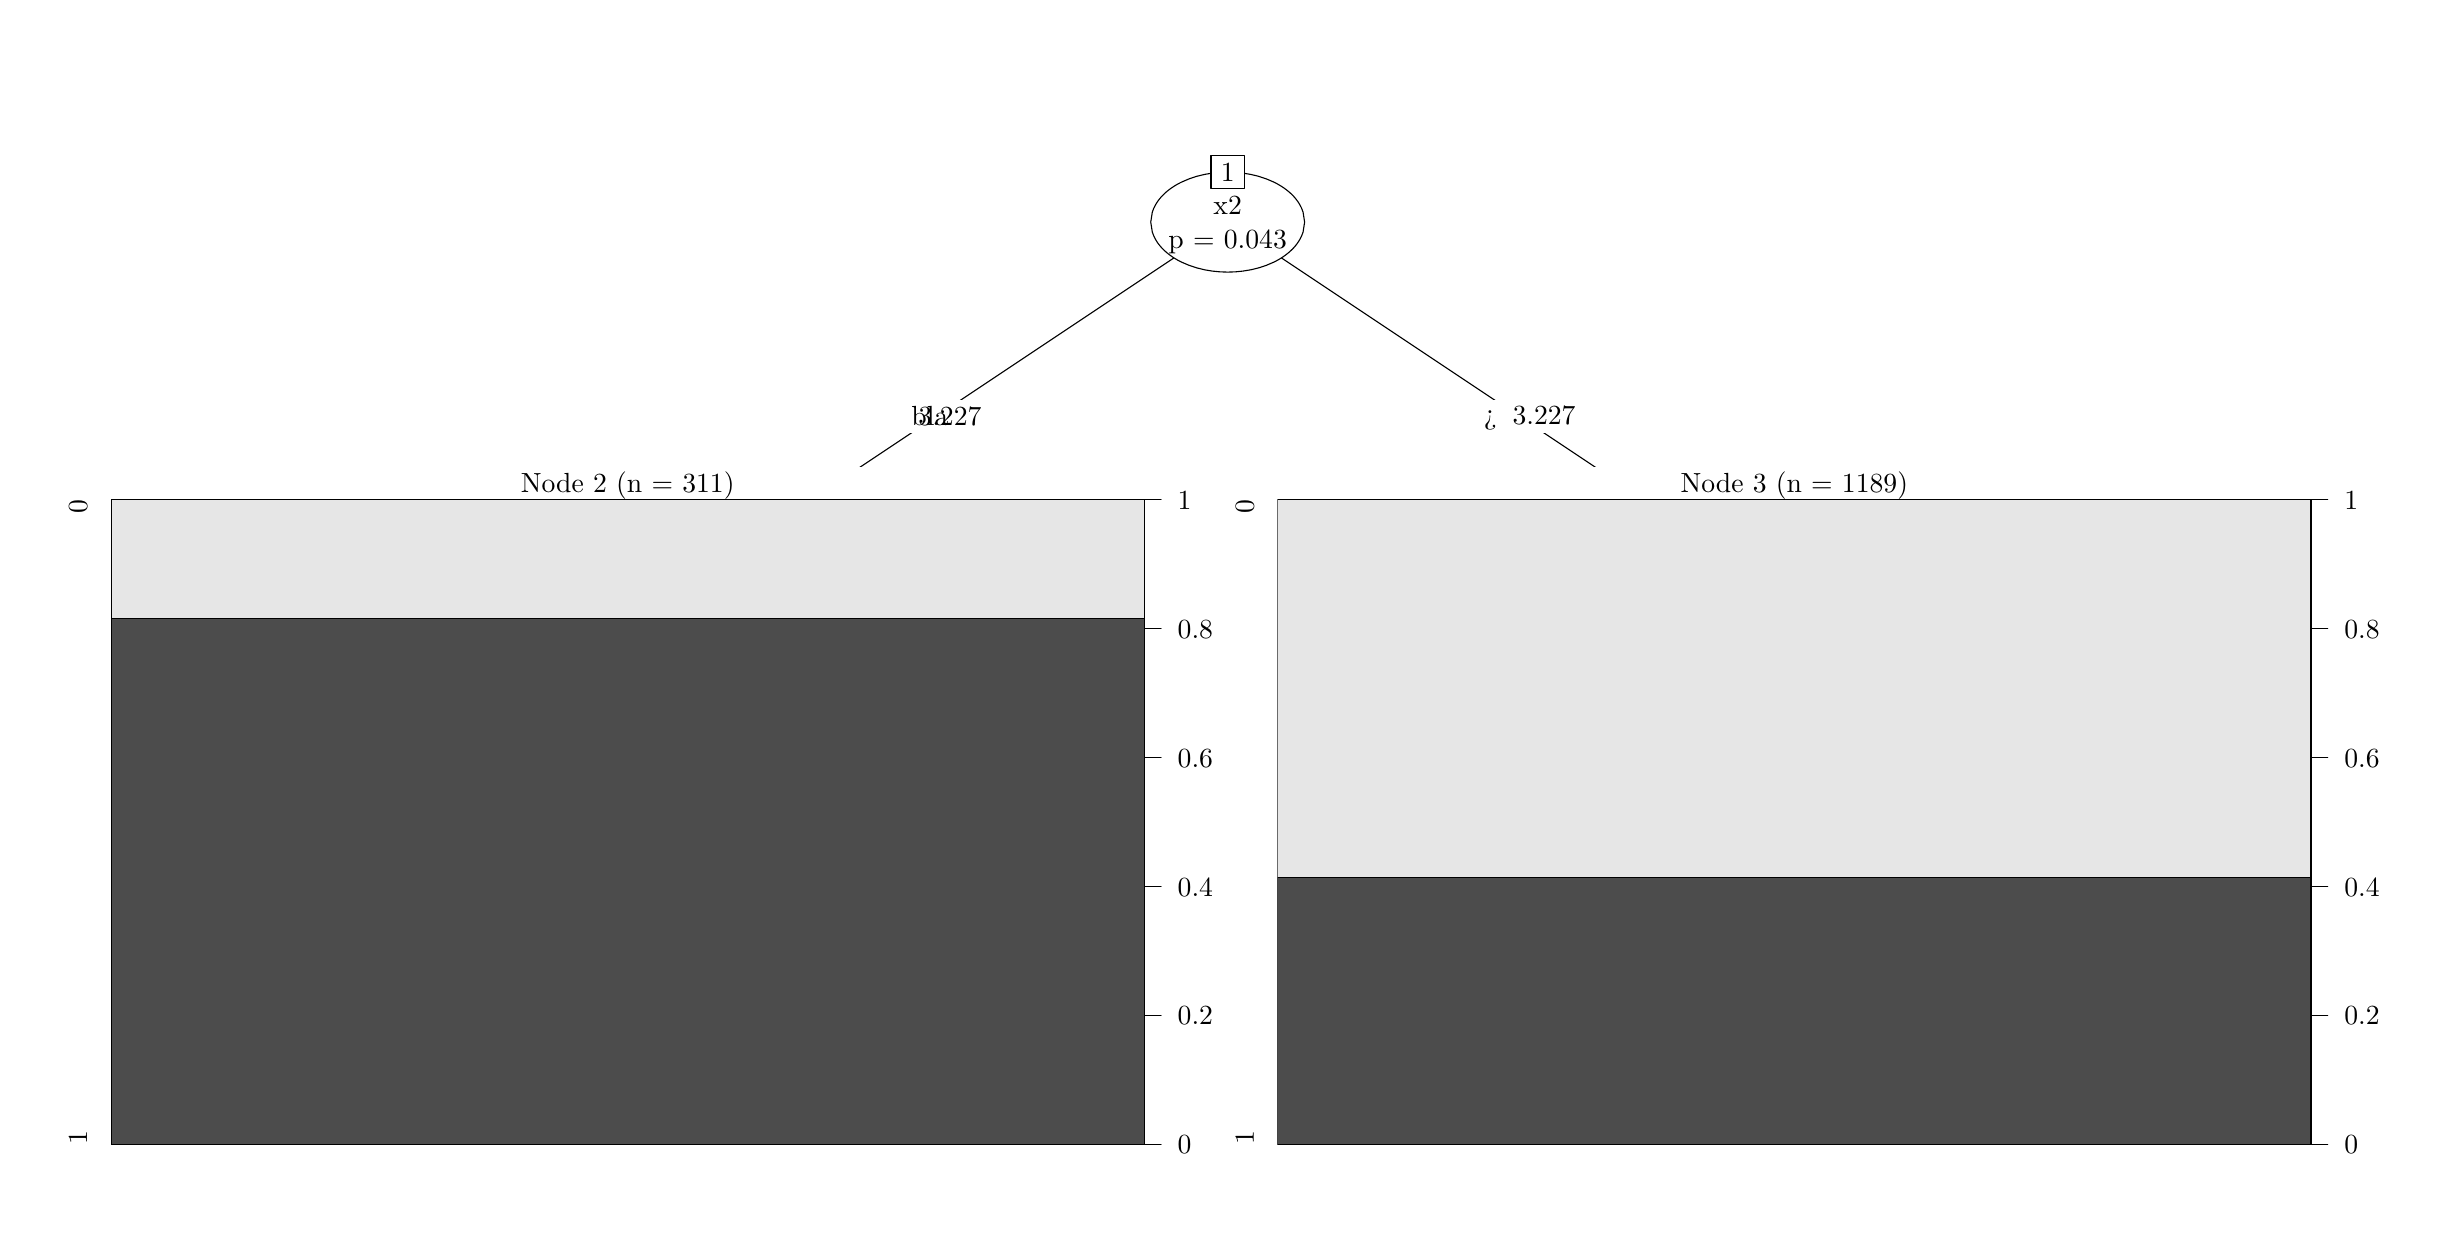
\begin{tikzpicture}[x=1pt,y=1pt]
\definecolor{fillColor}{RGB}{255,255,255}
\path[use as bounding box,fill=fillColor,fill opacity=0.00] (0,0) rectangle (867.24,433.62);
\begin{scope}
\path[clip] (  0.00,  0.00) rectangle (867.24,433.62);
\definecolor{drawColor}{RGB}{0,0,0}

\path[draw=drawColor,line width= 0.4pt,line join=round,line cap=round] (433.62,363.36) --
	(222.83,222.83);

\path[draw=drawColor,line width= 0.4pt,line join=round,line cap=round] (433.62,363.36) --
	(644.41,222.83);
\definecolor{fillColor}{RGB}{255,255,255}

\path[draw=drawColor,line width= 0.4pt,line join=round,line cap=round,fill=fillColor] (405.82,363.36) --
	(406.38,366.95) --
	(406.93,368.42) --
	(407.49,369.52) --
	(408.05,370.44) --
	(408.60,371.23) --
	(409.16,371.94) --
	(409.71,372.58) --
	(410.27,373.16) --
	(410.83,373.70) --
	(411.38,374.20) --
	(411.94,374.66) --
	(412.49,375.10) --
	(413.05,375.51) --
	(413.60,375.90) --
	(414.16,376.26) --
	(414.72,376.60) --
	(415.27,376.93) --
	(415.83,377.24) --
	(416.38,377.53) --
	(416.94,377.81) --
	(416.94,377.81) --
	(419.72,379.00) --
	(422.50,379.92) --
	(425.28,380.59) --
	(428.06,381.06) --
	(430.84,381.33) --
	(433.62,381.43) --
	(436.40,381.33) --
	(439.18,381.06) --
	(441.96,380.59) --
	(444.74,379.92) --
	(447.52,379.00) --
	(450.30,377.81) --
	(450.30,377.81) --
	(450.86,377.53) --
	(451.41,377.24) --
	(451.97,376.93) --
	(452.52,376.60) --
	(453.08,376.26) --
	(453.64,375.90) --
	(454.19,375.51) --
	(454.75,375.10) --
	(455.30,374.66) --
	(455.86,374.20) --
	(456.41,373.70) --
	(456.97,373.16) --
	(457.53,372.58) --
	(458.08,371.94) --
	(458.64,371.23) --
	(459.19,370.44) --
	(459.75,369.52) --
	(460.31,368.42) --
	(460.86,366.95) --
	(461.42,363.36) --
	(461.42,363.36) --
	(460.86,359.76) --
	(460.31,358.30) --
	(459.75,357.19) --
	(459.19,356.28) --
	(458.64,355.48) --
	(458.08,354.78) --
	(457.53,354.14) --
	(456.97,353.55) --
	(456.41,353.02) --
	(455.86,352.52) --
	(455.30,352.05) --
	(454.75,351.62) --
	(454.19,351.21) --
	(453.64,350.82) --
	(453.08,350.45) --
	(452.52,350.11) --
	(451.97,349.78) --
	(451.41,349.47) --
	(450.86,349.18) --
	(450.30,348.90) --
	(450.30,348.90) --
	(447.52,347.71) --
	(444.74,346.80) --
	(441.96,346.12) --
	(439.18,345.66) --
	(436.40,345.38) --
	(433.62,345.29) --
	(430.84,345.38) --
	(428.06,345.66) --
	(425.28,346.12) --
	(422.50,346.80) --
	(419.72,347.71) --
	(416.94,348.90) --
	(416.94,348.90) --
	(416.38,349.18) --
	(415.83,349.47) --
	(415.27,349.78) --
	(414.72,350.11) --
	(414.16,350.45) --
	(413.60,350.82) --
	(413.05,351.21) --
	(412.49,351.62) --
	(411.94,352.05) --
	(411.38,352.52) --
	(410.83,353.02) --
	(410.27,353.55) --
	(409.71,354.14) --
	(409.16,354.78) --
	(408.60,355.48) --
	(408.05,356.28) --
	(407.49,357.19) --
	(406.93,358.30) --
	(406.38,359.76) --
	(405.82,363.36) --
	cycle;

\node[text=drawColor,anchor=base,inner sep=0pt, outer sep=0pt, scale=  1.00] at (433.62,365.94) {x2};

\node[text=drawColor,anchor=base,inner sep=0pt, outer sep=0pt, scale=  1.00] at (433.62,353.89) {p = 0.043};

\path[draw=drawColor,line width= 0.4pt,line join=round,line cap=round,fill=fillColor] (427.60,375.40) rectangle (439.64,387.45);

\node[text=drawColor,anchor=base,inner sep=0pt, outer sep=0pt, scale=  1.00] at (433.62,377.98) {1};
\end{scope}
\begin{scope}
\path[clip] (  0.00,  0.00) rectangle (867.24,433.62);
\definecolor{fillColor}{RGB}{255,255,255}

\path[fill=fillColor] (311.80,287.07) rectangle (344.66,299.12);
\definecolor{drawColor}{RGB}{0,0,0}

\node[text=drawColor,anchor=base west,inner sep=0pt, outer sep=0pt, scale=  1.00] at (319.34,289.89) {bla};

\node[text=drawColor,anchor=base west,inner sep=0pt, outer sep=0pt, scale=  1.00] at (321.89,289.89) {3.227};
\end{scope}
\begin{scope}
\path[clip] (  0.00,  0.00) rectangle (867.24,433.62);
\definecolor{fillColor}{RGB}{255,255,255}

\path[fill=fillColor] (518.69,287.07) rectangle (559.33,299.12);
\definecolor{drawColor}{RGB}{0,0,0}

\node[text=drawColor,anchor=base west,inner sep=0pt, outer sep=0pt, scale=  1.00] at (526.24,290.08) {>};

\node[text=drawColor,anchor=base west,inner sep=0pt, outer sep=0pt, scale=  1.00] at (536.56,290.08) {3.227};
\end{scope}
\begin{scope}
\path[clip] (  0.00,  0.00) rectangle (867.24,433.62);
\definecolor{fillColor}{RGB}{255,255,255}

\path[fill=fillColor] ( 12.04, 30.11) rectangle (433.62,275.03);
\definecolor{drawColor}{RGB}{0,0,0}

\node[text=drawColor,anchor=base,inner sep=0pt, outer sep=0pt, scale=  1.00] at (216.81,265.56) {Node 2 (n = 311)};
\end{scope}
\begin{scope}
\path[clip] (  0.00,  0.00) rectangle (867.24,433.62);
\definecolor{drawColor}{RGB}{0,0,0}

\node[text=drawColor,rotate= 90.00,anchor=base west,inner sep=0pt, outer sep=0pt, scale=  1.00] at ( 21.51, 30.11) {1};

\node[text=drawColor,rotate= 90.00,anchor=base east,inner sep=0pt, outer sep=0pt, scale=  1.00] at ( 21.51,262.98) {0};

\path[draw=drawColor,line width= 0.4pt,line join=round,line cap=round] (403.51, 30.11) --
	(403.51,262.98);

\path[draw=drawColor,line width= 0.4pt,line join=round,line cap=round] (403.51, 30.11) -- (409.53, 30.11);

\path[draw=drawColor,line width= 0.4pt,line join=round,line cap=round] (403.51, 76.69) -- (409.53, 76.69);

\path[draw=drawColor,line width= 0.4pt,line join=round,line cap=round] (403.51,123.26) -- (409.53,123.26);

\path[draw=drawColor,line width= 0.4pt,line join=round,line cap=round] (403.51,169.83) -- (409.53,169.83);

\path[draw=drawColor,line width= 0.4pt,line join=round,line cap=round] (403.51,216.41) -- (409.53,216.41);

\path[draw=drawColor,line width= 0.4pt,line join=round,line cap=round] (403.51,262.98) -- (409.53,262.98);

\node[text=drawColor,anchor=base west,inner sep=0pt, outer sep=0pt, scale=  1.00] at (415.55, 26.67) {0};

\node[text=drawColor,anchor=base west,inner sep=0pt, outer sep=0pt, scale=  1.00] at (415.55, 73.24) {0.2};

\node[text=drawColor,anchor=base west,inner sep=0pt, outer sep=0pt, scale=  1.00] at (415.55,119.82) {0.4};

\node[text=drawColor,anchor=base west,inner sep=0pt, outer sep=0pt, scale=  1.00] at (415.55,166.39) {0.6};

\node[text=drawColor,anchor=base west,inner sep=0pt, outer sep=0pt, scale=  1.00] at (415.55,212.96) {0.8};

\node[text=drawColor,anchor=base west,inner sep=0pt, outer sep=0pt, scale=  1.00] at (415.55,259.54) {1};
\end{scope}
\begin{scope}
\path[clip] ( 30.11, 30.11) rectangle (403.51,262.98);
\definecolor{drawColor}{RGB}{0,0,0}

\path[draw=drawColor,line width= 0.4pt,line join=round,line cap=round] ( 30.11, 30.11) rectangle (403.51,262.98);
\definecolor{fillColor}{gray}{0.30}

\path[draw=drawColor,line width= 0.4pt,line join=round,line cap=round,fill=fillColor] ( 30.11, 30.11) rectangle (403.51,220.30);
\definecolor{fillColor}{RGB}{230,230,230}

\path[fill=fillColor] ( 30.11,220.30) rectangle (403.51,262.98);

\path[draw=drawColor,line width= 0.4pt,line join=round,line cap=round] ( 30.11, 30.11) rectangle (403.51,262.98);
\end{scope}
\begin{scope}
\path[clip] (  0.00,  0.00) rectangle (867.24,433.62);
\definecolor{fillColor}{RGB}{255,255,255}

\path[fill=fillColor] (433.62, 30.11) rectangle (855.20,275.03);
\definecolor{drawColor}{RGB}{0,0,0}

\node[text=drawColor,anchor=base,inner sep=0pt, outer sep=0pt, scale=  1.00] at (638.38,265.56) {Node 3 (n = 1189)};
\end{scope}
\begin{scope}
\path[clip] (  0.00,  0.00) rectangle (867.24,433.62);
\definecolor{drawColor}{RGB}{0,0,0}

\node[text=drawColor,rotate= 90.00,anchor=base west,inner sep=0pt, outer sep=0pt, scale=  1.00] at (443.09, 30.11) {1};

\node[text=drawColor,rotate= 90.00,anchor=base east,inner sep=0pt, outer sep=0pt, scale=  1.00] at (443.09,262.98) {0};

\path[draw=drawColor,line width= 0.4pt,line join=round,line cap=round] (825.08, 30.11) --
	(825.08,262.98);

\path[draw=drawColor,line width= 0.4pt,line join=round,line cap=round] (825.08, 30.11) -- (831.11, 30.11);

\path[draw=drawColor,line width= 0.4pt,line join=round,line cap=round] (825.08, 76.69) -- (831.11, 76.69);

\path[draw=drawColor,line width= 0.4pt,line join=round,line cap=round] (825.08,123.26) -- (831.11,123.26);

\path[draw=drawColor,line width= 0.4pt,line join=round,line cap=round] (825.08,169.83) -- (831.11,169.83);

\path[draw=drawColor,line width= 0.4pt,line join=round,line cap=round] (825.08,216.41) -- (831.11,216.41);

\path[draw=drawColor,line width= 0.4pt,line join=round,line cap=round] (825.08,262.98) -- (831.11,262.98);

\node[text=drawColor,anchor=base west,inner sep=0pt, outer sep=0pt, scale=  1.00] at (837.13, 26.67) {0};

\node[text=drawColor,anchor=base west,inner sep=0pt, outer sep=0pt, scale=  1.00] at (837.13, 73.24) {0.2};

\node[text=drawColor,anchor=base west,inner sep=0pt, outer sep=0pt, scale=  1.00] at (837.13,119.82) {0.4};

\node[text=drawColor,anchor=base west,inner sep=0pt, outer sep=0pt, scale=  1.00] at (837.13,166.39) {0.6};

\node[text=drawColor,anchor=base west,inner sep=0pt, outer sep=0pt, scale=  1.00] at (837.13,212.96) {0.8};

\node[text=drawColor,anchor=base west,inner sep=0pt, outer sep=0pt, scale=  1.00] at (837.13,259.54) {1};
\end{scope}
\begin{scope}
\path[clip] (451.69, 30.11) rectangle (825.08,262.98);
\definecolor{drawColor}{RGB}{0,0,0}

\path[draw=drawColor,line width= 0.4pt,line join=round,line cap=round] (451.69, 30.11) rectangle (825.08,262.98);
\definecolor{fillColor}{gray}{0.30}

\path[draw=drawColor,line width= 0.4pt,line join=round,line cap=round,fill=fillColor] (451.69, 30.11) rectangle (825.08,126.67);
\definecolor{fillColor}{RGB}{230,230,230}

\path[fill=fillColor] (451.69,126.67) rectangle (825.08,262.98);

\path[draw=drawColor,line width= 0.4pt,line join=round,line cap=round] (451.69, 30.11) rectangle (825.08,262.98);
\end{scope}
\end{tikzpicture}
